\clearpage
\section{Modelo de datos (Supabase / PostgreSQL)}
\label{sec:datos}
\subsection{Fuentes y alcance}
El modelo revisado se obtiene de las migraciones SQL locales, no de una exportación
remota. Las seis migraciones del scraper se encuentran en
\nolinkurl{tmp_scraper_repo/supabase/migrations/}: catálogo inicial (31-08), ubicación
(02-09), enriquecimiento y controles de organizadores (11-09), estado de reescritura
(12-09), publicación atómica (21-09) e interacciones (24-09), todas de 2026.
La aplicación añade \nolinkurl{20261024000100_password_reset_tokens.sql} y
\nolinkurl{20261024000200_avatars_bucket.sql} en su propio directorio
\nolinkurl{supabase/migrations/}. Son conjuntos de componentes diferentes.
El DBML y diccionario base están en \nolinkurl{tmp_scraper_repo/docs/evento_cultural_modelo.dbml}
y \nolinkurl{tmp_scraper_repo/docs/DATABASE.md} (03-10-2026). Se contrastaron con SQL;
no incluyen password\_reset\_tokens del frontend. La copia integrada editable
\nolinkurl{Diagramas/modelo_datos.dbml} añade esa tabla sin modificar las fuentes originales.
Se corrige la afirmación general de que no existían migraciones locales: pueden haber
faltado en un entregable antiguo, pero están disponibles en las copias aquí revisadas.
No se comprobó cuáles se aplicaron a Supabase ni qué cambios manuales posteriores existen.

\clearpage
\subsection{ER dividido por dominio}
Para legibilidad se muestran claves y relaciones principales, no cada columna. El inventario
y diccionario resumido siguientes completan la lectura. \texttt{auth\_users} es exclusivamente
el alias conceptual de Mermaid para la tabla real \texttt{auth.users}, gestionada por Supabase Auth;
no es una tabla adicional en public ni una copia de credenciales.
\begin{figure}[H]\centering
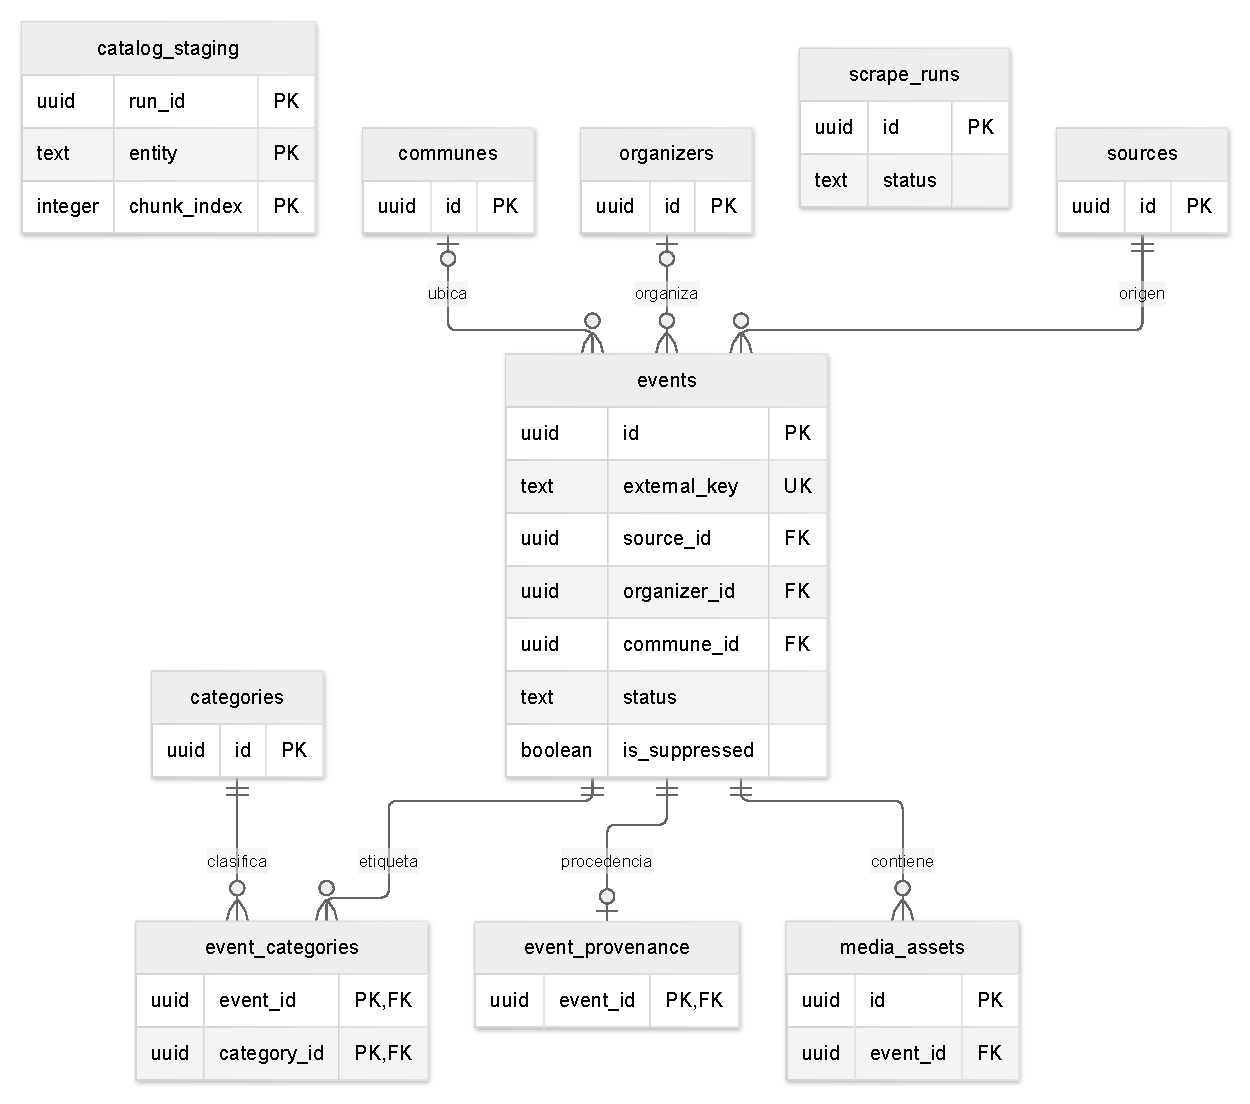
\includegraphics[width=\textwidth,height=0.59\textheight,keepaspectratio]{06_modelo_er.pdf}
\caption{ER del catálogo local: claves, opcionalidad y relaciones principales.}\label{fig:er}
\end{figure}
\clearpage
\begin{figure}[H]\centering
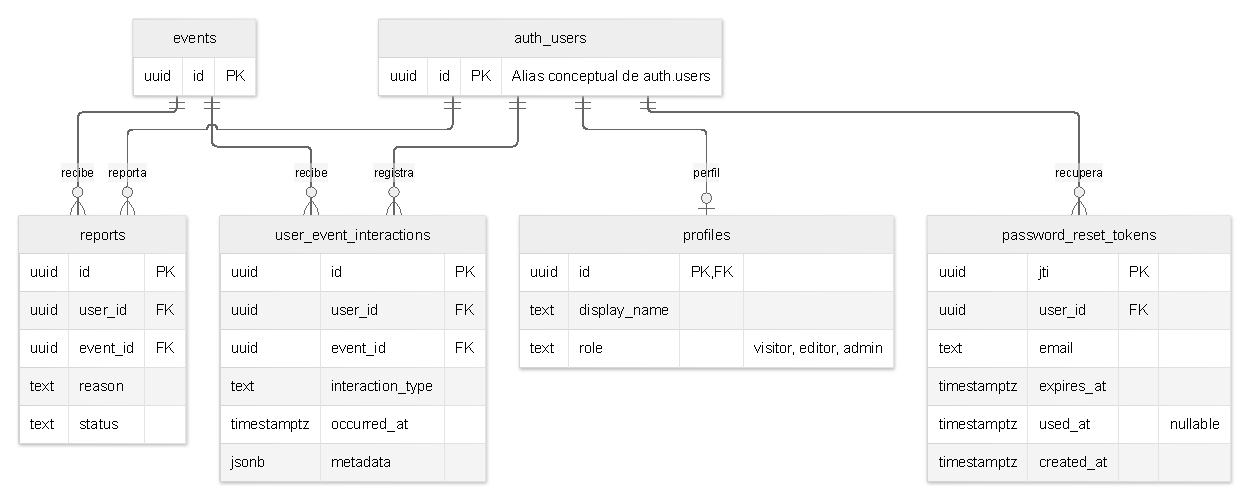
\includegraphics[width=\textwidth,height=0.70\textheight,keepaspectratio]{08_identidad_recuperacion.pdf}
\caption{Identidad, perfiles, interacciones y recuperación; auth\_users representa auth.users.}\label{fig:er-identidad}
\end{figure}

\subsection{Inventario y diccionario resumido}
Todas las tablas siguientes son del esquema public salvo auth.users y los objetos de Storage.
No se fija un número de columnas de events como propiedad del esquema remoto.
\begin{longtable}{p{4.0cm}p{9.6cm}}
\caption{Entidades y claves contrastadas con SQL local.}\label{tab:tablas}\\
\toprule Entidad & Claves, finalidad y alcance \\\midrule\endfirsthead
\toprule Entidad & Claves, finalidad y alcance \\\midrule\endhead
sources & id UUID PK, name único sin distinguir mayúsculas; fuente, website\_url, is\_active y last\_seen\_at. \\
organizers & id UUID PK, name único; entity\_type e is\_blocked, blocked\_reason, blocked\_at. La publicación busca por nombre: no hay FK demostrada a usuario propietario. \\
communes & id UUID PK; name, region y country, identidad territorial normalizada. \\
categories & id UUID PK, name único; event\_categories une evento/categoría con PK compuesta y dos FK. \\
events & id UUID PK; external\_key única; source\_id obligatoria; organizer\_id y commune\_id opcionales. Datos de ficha, fechas, location, location\_precision/source, coordenadas, status, is\_suppressed, marcas de extracción y actualización. El ER resume claves, no el diccionario completo de columnas. \\
media\_assets & id UUID PK, event\_id FK, url, media\_type, is\_primary; unicidad por evento/URL. \\
\nolinkurl{event_provenance} & event\_id PK/FK a events; original\_url, source\_description, ocr\_text, is\_rewritten y updated\_at; la migración del 12-09 expone ese estado en match\_existing\_events, no añade otra columna; información privada de procedencia. \\
scrape\_runs & id UUID PK; started\_at, finished\_at, status (running/succeeded/failed), events\_count, error\_message y metadata. Sin FK a events en el SQL revisado. \\
catalog\_staging & PK (run\_id, entity, chunk\_index), payload JSONB y created\_at; no se dibuja una FK de run\_id a scrape\_runs porque el SQL no la declara. publish\_staged\_catalog aplica la carga transaccional. \\
auth.users & Tabla externa administrada por Auth; id UUID referenciada por los datos de cuenta. auth\_users es solo su nombre conceptual en el dibujo. \\
profiles & id PK/FK a auth.users; display\_name, role (visitor/editor/admin) y marcas de tiempo. La migración inicial concede actualizar display\_name, no role, a authenticated. \\
\nolinkurl{user_event_interactions} & id PK, user\_id FK a auth.users y event\_id FK a events; interaction\_type, occurred\_at, metadata JSONB. La migración del 24-09 migra favorites a interested y elimina favorites. \\
reports & id PK, user\_id y event\_id FK; reason, status (pending/reviewed/resolved) y marcas de tiempo. Tabla disponible no acredita un flujo ciudadano completo. \\
\nolinkurl{password_reset_tokens} & jti UUID PK; user\_id UUID FK a auth.users con ON DELETE CASCADE; email TEXT NOT NULL; expires\_at TIMESTAMPTZ NOT NULL; used\_at TIMESTAMPTZ nullable; created\_at TIMESTAMPTZ NOT NULL DEFAULT now(). Índices por email y expires\_at. \\
Storage avatars & No es una tabla de catálogo: bucket en storage.buckets y objetos en storage.objects. Migración local propone lectura pública y escrituras de authenticated bajo carpeta auth.uid(). No acredita políticas aplicadas remotamente. \\
\bottomrule\end{longtable}
Los UUID v5 deterministas son una decisión del exportador del scraper, no una restricción
global del tipo UUID en PostgreSQL. La función publicar-evento utiliza crypto.randomUUID()
y claves externas org:usuario:tiempo:sufijo; no se afirma que toda alta tenga UUID v5.

\subsection{Autorización de Fase 3 y recuperación}
La administración usa profiles.role y una comprobación de proveedor en admin-eventos,
además del guard cliente. La publicación usa user\_metadata.rol=organizador y crea status=draft.
Ese metadata de autoservicio no demuestra propiedad administrativa ni relación estable
usuario--organizador; tampoco debe confundirse con profiles.role.

password\_reset\_tokens registra el jti del token temporal emitido por reset-password-request.
reset-password-confirm valida token, vencimiento y marca de uso antes de completar el cambio.
La migración habilita RLS sin crear políticas, pero no contiene un REVOKE/GRANT explícito;
no basta para describir todos los privilegios efectivos remotos. Tampoco se certifica
consumo atómico ante concurrencia ni recuperación extremo a extremo mediante inspección estática.
La migración del bucket avatars es separada de la recuperación y del scraper.

\subsection{Vista public\_event\_catalog, permisos y RLS}
\nolinkurl{20260911000100_content_enrichment_and_organizer_controls.sql} declara:
\begin{minipage}{\linewidth}
\begin{lstlisting}
create view public.public_event_catalog
with (security_invoker = true) as
select e.*, o.name as organizer_name, s.name as source_name
from public.events e
join public.sources s on s.id = e.source_id
left join public.organizers o on o.id = e.organizer_id
where e.status = 'published' and not e.is_suppressed;
revoke all on public.public_event_catalog from public;
grant select on public.public_event_catalog
  to anon, authenticated, service_role;
\end{lstlisting}
\end{minipage}
La misma migración define RLS en events para status published, no suprimido y
\texttt{not public.is\_organizer\_blocked(organizer\_id)}; modifica las políticas de
organizers, event\_categories y media\_assets. La función is\_organizer\_blocked es
SECURITY DEFINER con concesión EXECUTE a anon/authenticated/service\_role.
La migración inicial concede SELECT en tablas base y la del 11-09 restringe la lectura
de organizers a columnas identificadas. La política de sources exige is\_active.

\textbf{No existe herencia automática de RLS por el mero hecho de crear una vista.}
Según CREATE VIEW de PostgreSQL (referencias), security\_invoker=true aplica los
privilegios y políticas del invocador sobre las relaciones subyacentes; por defecto
se usan los del propietario. Aquí se acredita el mecanismo en SQL local, no su despliegue.
service\_role puede eludir RLS y no equivale al usuario público. Deben verificarse versión
compatible (PostgreSQL 15 o posterior), propietario, reloptions, definición efectiva,
permisos base/funciones y pg\_policies; además de pruebas con identidades separadas.
No se consultó el esquema remoto. No se concluye vulnerabilidad ni conformidad por esa limitación.

\section{Diagramas UML y flujos}
\label{sec:uml}
\subsection{Casos de uso actuales}
\begin{figure}[H]\centering
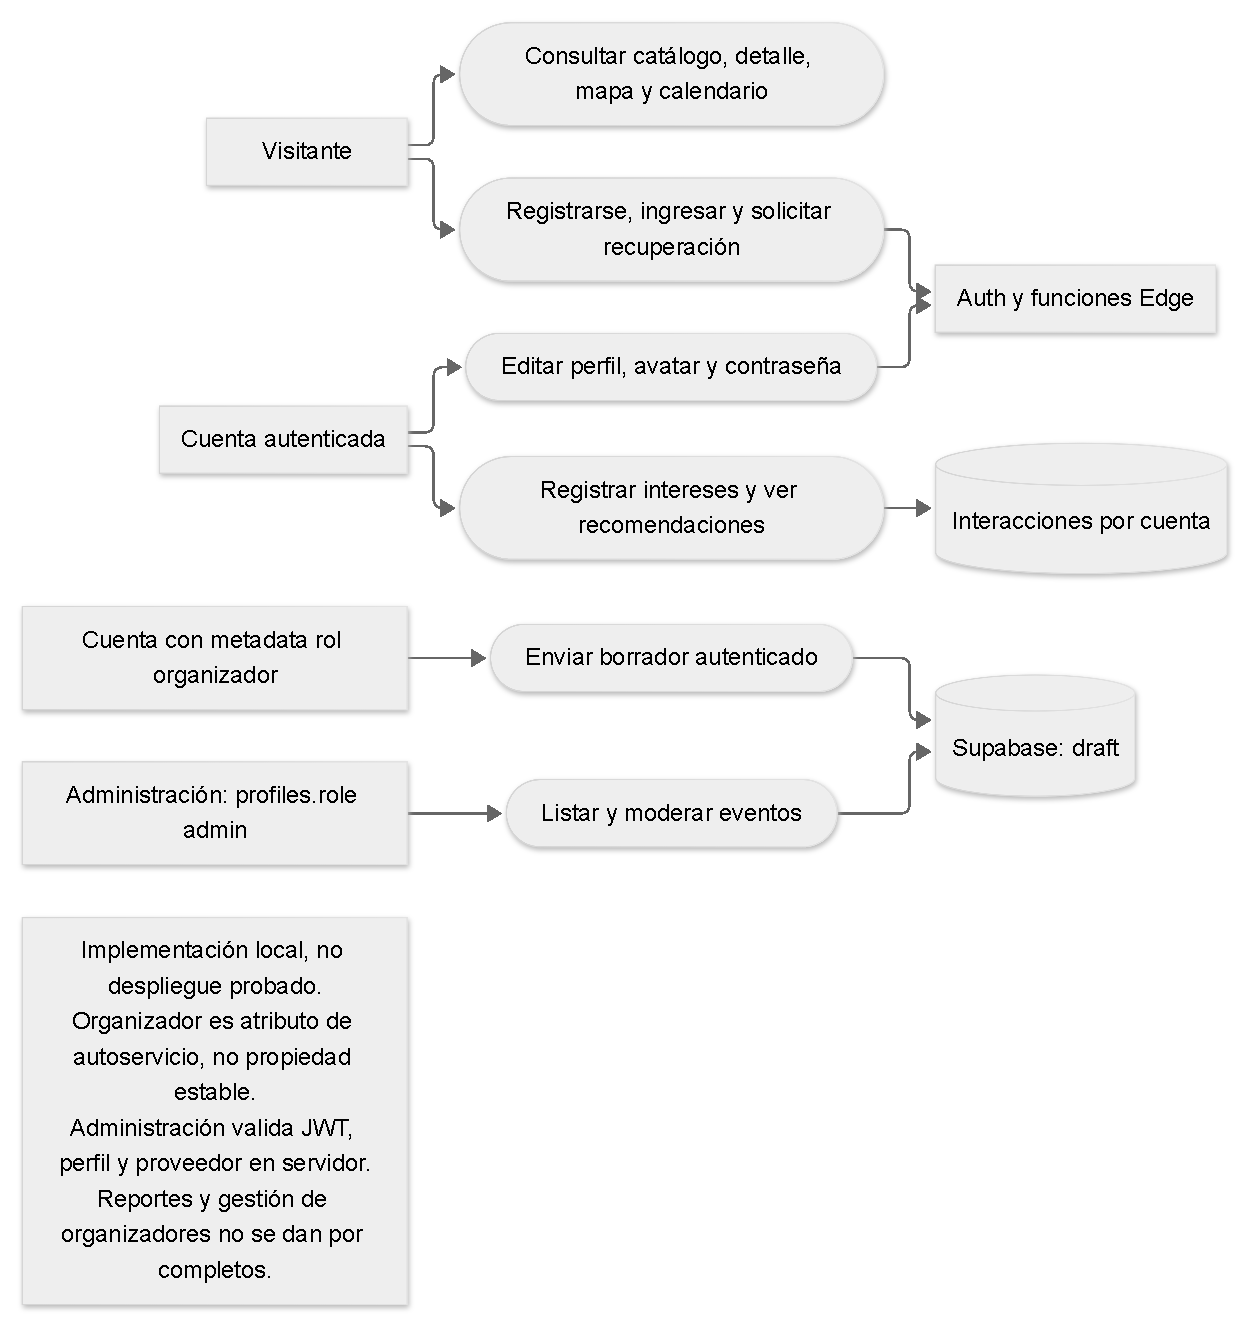
\includegraphics[width=\textwidth,height=0.67\textheight,keepaspectratio]{03_casos_de_uso.pdf}
\caption{Casos de uso locales; conceptual, no certificación de despliegue.}\label{fig:uc}
\end{figure}
El visitante descubre eventos y accede al registro; el usuario autenticado gestiona
cuenta, perfil e intereses. La condición de organizador es metadata autodeclarada para
enviar borradores. El administrador usa su rol en profiles para moderar. Correo y OAuth
tienen integración local; recepción, configuración y recorridos completos no se dan por probados.
GitHub Actions y NVIDIA son actores técnicos del scraper, representados en su pipeline,
no roles ciudadanos. Reportes y administración de organizadores no se presentan como completos.

\subsection{Registro, sesión, publicación y moderación}
\begin{figure}[H]\centering
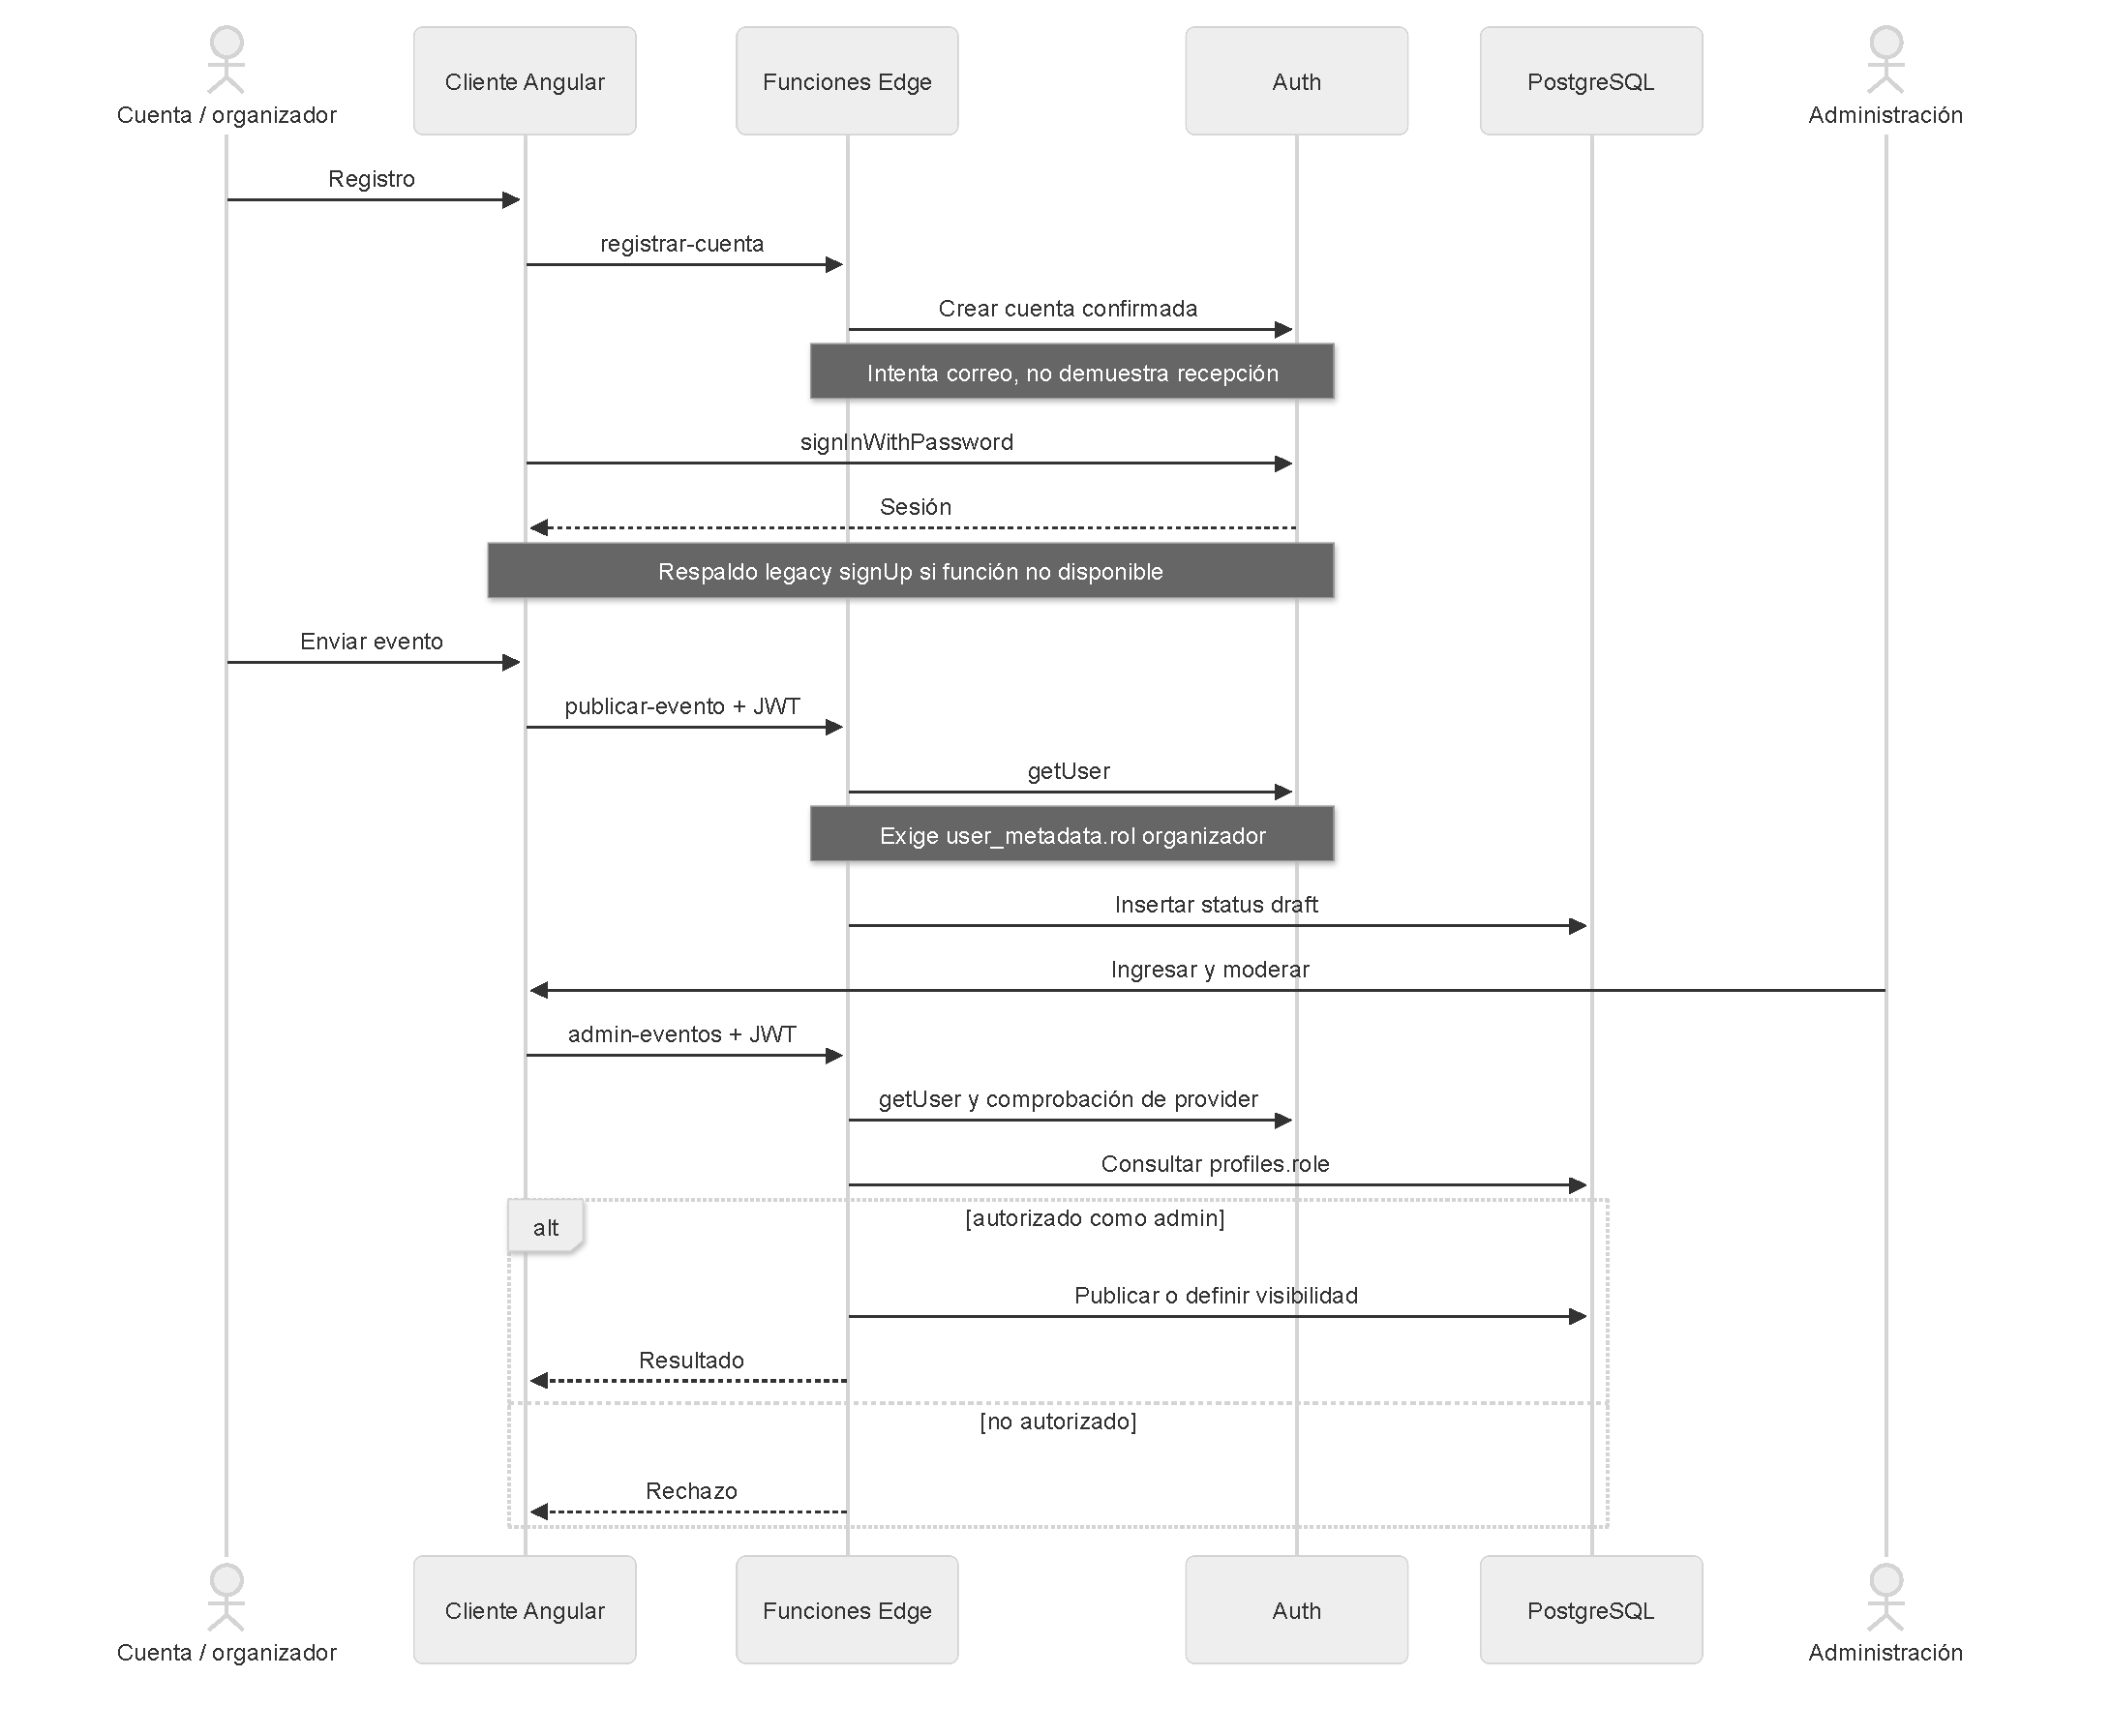
\includegraphics[width=\textwidth,height=0.70\textheight,keepaspectratio]{04_secuencia.pdf}
\caption{Secuencia resumida de cuenta y moderación.}\label{fig:seq}
\end{figure}
El cliente solicita registrar-cuenta; la función crea una cuenta confirmada mediante
Admin API e intenta enviar bienvenida. Después el cliente inicia sesión con contraseña.
La confirmación de cuenta no prueba propiedad del buzón ni recepción del correo. Existe
respaldo legacy signUp si falla la disponibilidad de la función. Para publicar, la función
valida JWT y metadata de organizador antes de insertar draft. Para moderar, admin-eventos
valida identidad, proveedor y profiles.role antes de publicar o cambiar is\_suppressed.
La secuencia representa el flujo nominal y el rechazo administrativo, no una ejecución
registrada. La explicación de extracción y enriquecimiento está en la Sección~\ref{sec:scraper}.

\subsection{Clases y componentes}
El diagrama de componentes aparece en la Figura~\ref{fig:comp}. Las clases siguientes
proceden del núcleo local del scraper; las relaciones son dependencias conceptuales,
no atributos o métodos traducidos inventados. Se corrigen PipelineState y NvidiaService
por los nombres observados StateStore, DetailCache y NvidiaContentEnricher.
\begin{figure}[H]\centering
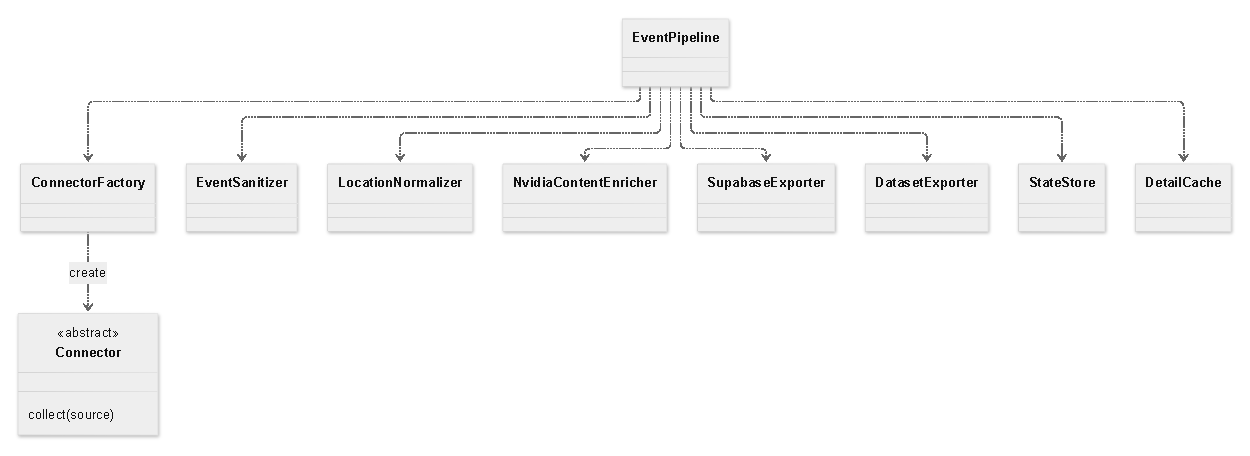
\includegraphics[width=\textwidth,height=0.66\textheight,keepaspectratio]{05_clases.pdf}
\caption{Clases locales y dependencias principales del scraper.}\label{fig:cls}
\end{figure}
Los fuentes Mermaid se incluyen en Diagramas/. El diagrama de casos de uso es conceptual:
si se exige notación UML estricta debe ratificarse la notación con el docente; no se
presenta esa ratificación como ya realizada.
